\documentclass{article}
\usepackage{graphicx}
\usepackage{amsmath}
\usepackage{amssymb}
\usepackage[a4paper, margin=.2in]{geometry}

\begin{document}
let's make our RC phase shiftter with passive component

\begin{figure}[h]
    \centering
    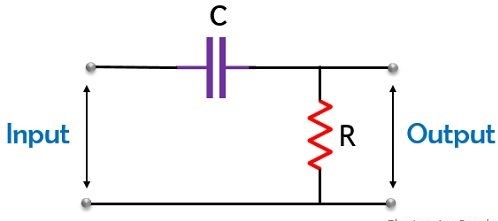
\includegraphics[width=.4\textwidth]{RC_phasse_shift.jpg}
\end{figure}
\[
\frac{V_{out}}{V_{in}} = \frac{R}{R - j \cdot X_C} = \frac{R}{R - \left( \frac{j}{\omega \cdot C} \right)} = \frac{1}{1 - \left( \frac{j}{\omega \cdot R \cdot C} \right)}
\]

\[
    \angle \phi = 0 - \tan ^{-1}(\frac{1}{\omega \cdot R \cdot C}) = \tan ^{-1}(\frac{X_C}{R})
\]

\[
    \angle \phi = 90^o \rightarrow 0^o
\]
cascadded three stages of RC phase shiftter, each one have \(60^o\) so overall is \(180^o\):
\begin{figure}[h]
    \centering
    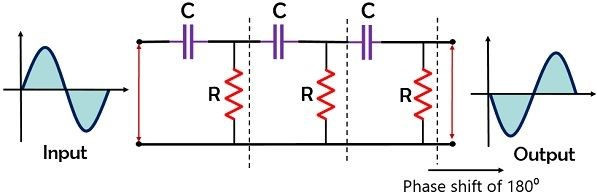
\includegraphics[width=.7\textwidth]{cascaddedRCPhaseShifter.jpg}
\end{figure}

Now to make overall phase shift is zero of loop gain we add inverting op-amp:
\begin{figure}[h]
    \centering
    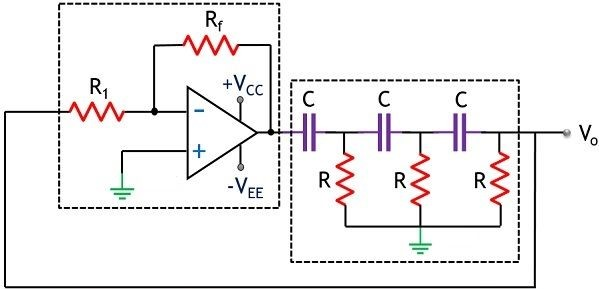
\includegraphics[width=.6\textwidth]{RC-phase-shift _oscillator-circuit.jpg}
\end{figure}

frequency of oscillation:
\[
\boxed{f=\frac{1}{2\pi RC\sqrt{2N}}}
\]
N: number of RC shiftter stages\\
in our case N=3:
\[
\boxed{f=\frac{1}{2\pi RC\sqrt{6}}}
\]
\end{document}